\documentclass[../598comp.tex]{subfiles}

\graphicspath{ {./lectures/images/}{./images/} }

\date{05-11}

\begin{document}

\section{05-11}

$\Sigma$ corresponds to the alphabet. $\Sigma^*$ represents finite words.
$\Sigma^\omega$ is the set of \ul{infinite words} over $\Sigma$.
\\\\
If $\Sigma = \{a, b\}$, $\Sigma^\omega$ is \ul{uncountable}. $\Sigma^\infty =
\Sigma^* \cup \Sigma^\omega$. A string in $\Sigma^\omega$ is countable, so positions in
the string can be indexed by $\NN$ i.e. countable.
\\\\
There is a natural partial order on $\Sigma^\infty$. $\alpha \leq \beta$ if $\alpha$
is a \ul{prefix} of $\beta$. Infinite strings cannot be compared.

First ordinal. Reflexivity is part of a partial order.

\begin{remark}
  We can define a \ul{metric} on $\Sigma^*$ by letting $d(x, y) = 2^{-n}$ where
  $n$ is the \ul{first} position where $x[n] != y[n]$. The longer the shared
  prefix the closer two words are. This is an ultrametric which means that it
  satisfies the following strengthened version of the triangle inequality
  \begin{gather*}
    d(x, z) \leq \max (d(x, y), d(y, z))
  \end{gather*}
  $\Sigma^\infty$ is the cauchy completion of $\Sigma^*$ and the metric
  naturally extends to $\Sigma^*$.
\end{remark}

Infinite strings are important for the verification of reactive systems. They
are designed to run forever so they have to talk about infinite computations.

\subsection{$\omega$ regular expressions.}

Let $E$ be a regular expression and $\epsilon \notin L(E)$.

$E^\omega$ is an $\omega$-regular expression.
\begin{gather*}
  L_\omega(E^\omega) \coloneqq \{w_1w_2w_3\cdots \ | \ w_i \in L(E)\}
\end{gather*}
where $L_\omega(F)$ is the $\omega$-language defined by the $\omega$ regular
expression $F$.

Let $E_i$ be regular xpressions and $F_i$ be regular expressions such that
$\epsilon \notin L(F_i)$.
\begin{gather*}
  E_1(F_1)^\omega + \cdots + E_n(F_n)^\omega
\end{gather*}
is a general $\omega$-regular expression.

$E^\omega = E E^\omega$ so $E^\omega$ is also an $\omega$-regular expression.
\\\\
When concatenating where $\alpha, \beta \in \Sigma^\omega$, $\alpha \beta = \alpha$.

\begin{definition}
  An $\omega$-language ($\subseteq \Sigma^\omega$) is $\omega$-regluar if defined
  by some $\omega$ regular expression. This $\omega$-regular expression may not
  be unique.
  \begin{note}
    $\cdot$ is concatenation. $+$ is union. $(.)^\omega$ is infinite repetition.
  \end{note}
\end{definition}

\subsection{$\omega$-automata}
Specifically non deterministic biichi automata. 
\begin{gather*}
  A = (Q, \Sigma, \delta, Q_0, F) \\
  \delta : Q \times \Sigma \to 2^Q \\
  s' \in \delta(s, a) \equiv s \to_a s'
\end{gather*}
Given a word $\sigma \in \Sigma^\omega$, a \ul{run} of $\omega$ in $A$ is an
infinite sequence of states $q_0, q_1, \cdots$ such that $q_0 \in Q_0, \ \forall
i \ q_i \to_{\sigma[i]} q_{i + 1}$.
% Given a word $\sigma \in \Sigma^\omega$, a \ul{run} of $\omega$ in $A$ is an
% infinite sequence of states $q_0, q_1, \cdots$ such that $q_0 \in Q_0, \ \forall
% i \ q_i \to_{\sigma[i]} q_{i + 1}$, where $\sigma[i]$ is the letter at
% position $i$ of $\sigma$. Everytime it hits an accept state it rings a bell.
\begin{gather*}
  inf(r) = \{q \ | \ q \ \text{occurs infinitely often in} r\}
\end{gather*}
A run is \ul{accepting} if it hits an accept state infinitely often. There are
only finitely many accept states so one of them has to be hit infinitely many times.
\begin{gather*}
  inf(r) \cap F \neq \varnothing
\end{gather*}
A word is accepted by $A$ if that word has some accepting run.
\begin{example}
  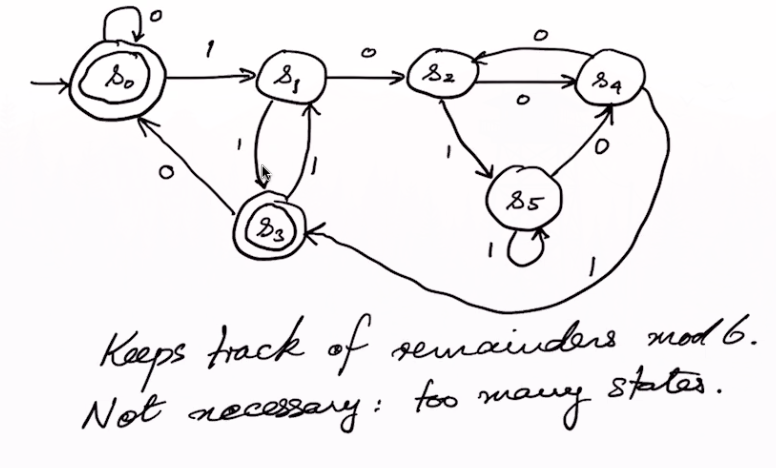
\includegraphics[width=\textwidth]{mod6machine}
  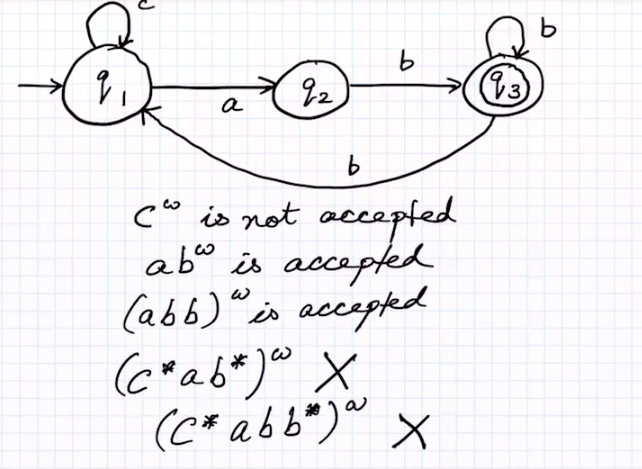
\includegraphics[width=\textwidth]{omega_regular_language}
  \begin{gather*}
    L_\omega(A) = c^*ab(b^+ + bc^*ab)^\omega
  \end{gather*}
  We see that it doesn't necessarily have to be periodic, but perhaps a periodic
  aspect to it. Get it to the start state first, then think of a pattern.
\end{example}

\begin{theorem}
  NBA's accept exactly the $\omega$-regular languages.
  \begin{proof}
    Show that any $\omega$-regular language can be captured by an NBA.
    \\\\
    Given $A_i = (Q_i, \Sigma, \delta_i, Q_{0, i}, F_i), \ i = 1, 2$ with $Q_1
    \cap Q_2 = \varnothing$. Then $A_1 + A_2 = (Q_1 \cup Q_2, \Sigma, \delta,
    Q_{0, 1} \cup Q_{0, 2}, F_1 \cup F_2)$. You can start either in start states
    of $A_1$ or $A_2$.
    \begin{gather*}
      \delta(q, a) = \delta_i(q, a) \ \text{if} \ q \in Q_i \\
      L_\omega (A_1 + A_2) = L_\omega(A_1) \cup L_\omega(A_2)
    \end{gather*}
    We are now considering $F^\omega$. We have an NFA for $F$ and assume that
    all the inital states are non accepting. $Q_0 \cap F = \varnothing$ and
    there are no \ul{incoming} transition to \ul{any} state in $Q_0$. You may
    worry that this will be too restricting on applicable NFAs. But if your
    NFA does not satisfy these assumptions we can modify it so that it does and
    defines the same language.
    \\\\
    Idea for doing this: Brand new unique start state. And then leave everything
    afterwards untouched.
    \\\\
    Given $A = (Q, \Sigma, \delta, Q_0, F)$. NBA $A' = (Q, \Sigma, \delta', Q_1,
    F')$. $L_\omega(A') = (L(A))^\omega$.
    The goal is to keep recognizing infinitely many words. So each time you hit
    an accept state, send it back to the start state.
    \\
    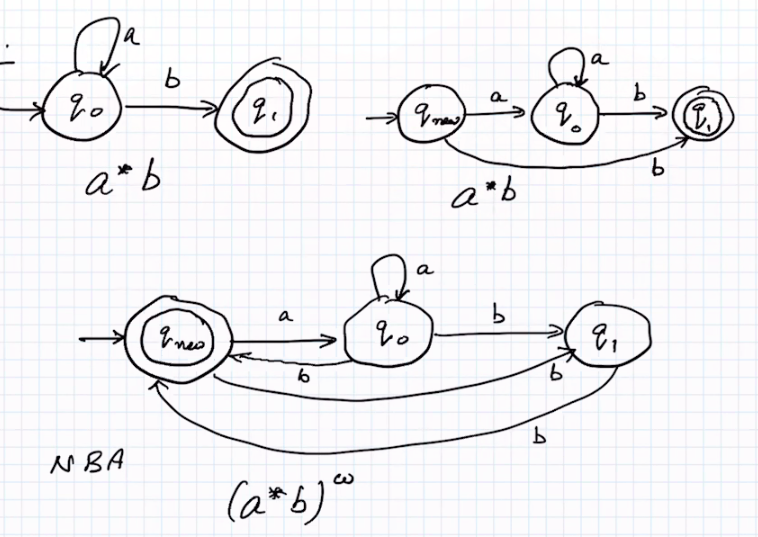
\includegraphics[width=\textwidth]{nfa_to_nba_example.png}
    \\\\
    Case three. NFA . NBA.
    \\
    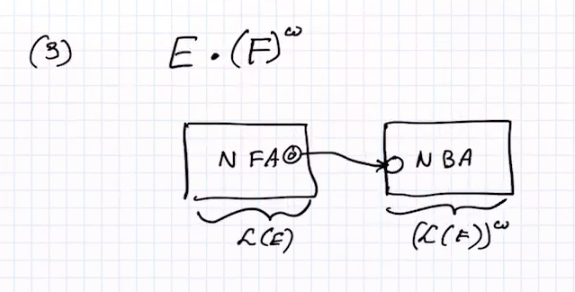
\includegraphics[width=\textwidth]{case_three_biichi.png}
    \\\\
    This proves that any language defined by an $\omega$-regexp can be
    recognized by an NBA. Cases are union of two omega regexp. extension of
    regexp to omega regexp. And concatenation of regexp with omega regexp.
  \end{proof}
\end{theorem}
\begin{theorem}
  Other direction
  \\\\
  Suppose $A = (Q, \Sigma, \delta, Q_0, F)$ NBA. Fix any 2 states. $A_{qp}
  \coloneqq (Q, \Sigma, \delta, \{q\}, \{p\})$. This converts it to an NFA. It
  is not meant to read omega words.
  \begin{gather*}
    L(A_{qp}) = L_{qp} = \{w \in \Sigma^* \ | \delta^*(q, w) \ni p\}
  \end{gather*}
  These are words that take you from $q$ to $p$.
  \\\\
  Now consider an accepted word $\sigma$ of $L_\omega(A)$ with an accepting run.
  It must hit sum $q \in F$ that appears infinitely often. Therefore
  \begin{gather*}
    \sigma = \underbrace{w_0}_{L_{q_0q}}\underbrace{w_1}_{L_{qq}}\underbrace{w_1}_{L_{qq}}\cdots
  \end{gather*}
  where $w_i$ are non empty. Any $\sigma$ the can be expressed like this has an
  accepting run. Therefore
  \begin{gather*}
    L_\omega(A) = \cup_{q_0 \in Q_0}\cup_{q \in F}L_{q_0q}\cdot(L_{qq} \setminus
    \{\epsilon\})^\omega
  \end{gather*}
  Therefore anything recognized by an NBA is described by an $\omega$-regular
  expression. Kleene's theorem for $\omega$-languages.
\end{theorem}

\begin{lemma}
  $L_\omega(A) \neq \varnothing$ iff $\exists$ a reachable accept state that
  belongs to a cycle.
\end{lemma}
$A_1 \equiv_F A_2$ they are the same as NFA. $L(A_1) = L(A_2)$. $A_1 \equiv_B
A_2$ they are the same as NBA. $L_\omega(A_1) = L_\omega(A_2)$.
\\\\
\begin{example}
  Does $\equiv_F \imply \equiv_B$? No!
  Does $\equiv_B \imply \equiv_F$? No!
  \\
  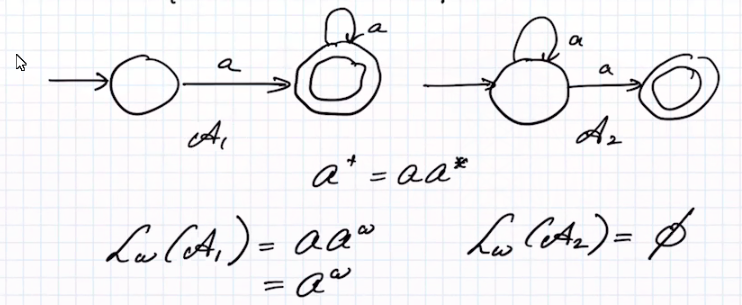
\includegraphics[width=\textwidth]{equiv_nfa_not_nba_example.png}
  \\
  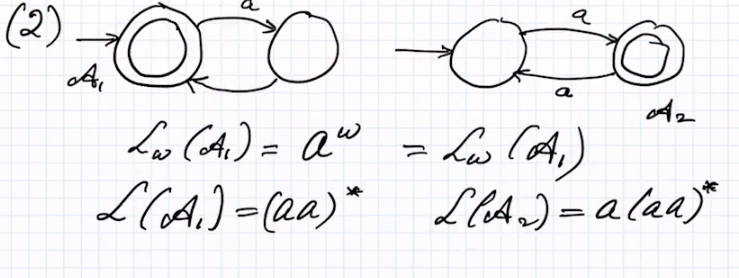
\includegraphics[width=\textwidth]{equiv_nba_not_nfa_example.png}
  Idea here is that it distinguishes even length from odd length, but infinity
  length is both even and odd.
\end{example}
\begin{theorem}
  NBAs and DBAs are not equivalent. There is no DBA that can recognize
  $(a+b)^*b^\omega$. This is what makes omega automata much trickier.
  \begin{proof}
    Suppose we have a DBA for this language. We can define $\delta^*$ as usual
    on the underlying DFA. Consider the word $b^\omega \in (a+b)^*b^\omega$
    \\\\
    Since $b^\omega$ is accepted, we must hit an accept state at some point.
    Therefore $\delta^*(q_0, b^{n_1})$ is an accept state. $b^{n_1}ab^\omega \in
    L$. This has to hit an accept state again after reading a. You can continue
    this process. Have to hit the same accept state twice. But then $\exists i,
    j, i < j$ where
    \begin{gather*}
      \delta^*(q_0, b^{n_1}ab^{n_2}\cdots ab^{n_i}) = \delta^*(q_0, b^{n_1}ab^{n_2}\cdots ab^{n_j})
    \end{gather*}
    But then there is a loop. So you can include infinitely many b in the
    language. Contradiction. So NBA are strictly more expressive than DBA.
  \end{proof}
\end{theorem}
Let $\alpha \in \Sigma^*\omega$ and define $\alpha|_n \in \Sigma^*$ to be the
length of $n$ finite prefix.
\begin{definition}
  For $W \subseteq \Sigma^*$ we define $\vec{W} = \{\alpha \in \Sigma^\omega \ |
  \exists \ \text{infinitely many} \ n \in \NN s.t. \ \alpha|_n \in W\}$
  Words where you can always make the prefix in $W$ longer. $\vec{W}$ is called
  a \ul{limit} language.
\end{definition}
\begin{theorem}
  An $\omega$-regular language $L$ is recognizable by a deterministic BA iff there
  is a \ul{regular} language $W$ such that $L = \vec{W}$.
  \begin{proof}
    DIY
  \end{proof}
\end{theorem}
\begin{theorem}
  DBA are closed under complement.
  \\\\
  If $A$ is a DBA, $\exists$ an NBA $A'$ such that $L_\omega(A') =
  \Sigma^*\omega \setminus L(A)$.
  \\\\
  $A' = (Q', \Sigma, \delta', Q_0', F'). A = (Q, \Sigma, \delta, Q_0, F)$. 
  \begin{gather*}
    Q' = (Q \times \{0\}) \cup ((Q \setminus F) \cup \{1\}) \\
    Q_0' = Q_0 \times \{0\} \\
  \end{gather*}
\end{theorem}
\end{document}